% Created 2020-03-19 Thu 10:12
% Intended LaTeX compiler: pdflatex
\documentclass[presentation]{beamer}
\usepackage[utf8]{inputenc}
\usepackage[T1]{fontenc}
\usepackage{graphicx}
\usepackage{grffile}
\usepackage{longtable}
\usepackage{wrapfig}
\usepackage{rotating}
\usepackage[normalem]{ulem}
\usepackage{amsmath}
\usepackage{textcomp}
\usepackage{amssymb}
\usepackage{capt-of}
\usepackage{hyperref}
\RequirePackage{fancyvrb}
\DefineVerbatimEnvironment{verbatim}{Verbatim}{fontsize=\scriptsize}
\usetheme{metropolis}
\usecolortheme{}
\usefonttheme{}
\useinnertheme{}
\useoutertheme{}
\author{Petru Rebeja, Marius Apetrii}
\date{19 Martie 2020}
\title{Tehnici Avansate de Programare}
\subtitle{Fluxul de lucru cu Git și principiile SOLID}
\institute[UAIC]{Facultatea de Matematică\\Universitatea Alexandru Ioan Cuza, Iași}
\hypersetup{
 pdfauthor={Petru Rebeja, Marius Apetrii},
 pdftitle={Tehnici Avansate de Programare},
 pdfkeywords={},
 pdfsubject={},
 pdfcreator={Emacs 26.3 (Org mode 9.3.4)},
 pdflang={Romanian}}
\begin{document}

\maketitle
\section{Introducere}
\label{sec:org1cca4fe}
\begin{frame}[label={sec:org34ecb77}]{Informații}
\begin{center}
Link-ul către spațiul Slack dedicat cursului va fi dezactivat azi.
\end{center}
\end{frame}
\begin{frame}[label={sec:org1e7e04b},fragile]{Recapitulare}
 \begin{itemize}
\item \texttt{Garbage collector}
\item \texttt{IDisposable}
\end{itemize}
\end{frame}
\begin{frame}[label={sec:org658104d},fragile]{Despre ce vom discuta azi}
 \begin{itemize}
\item Fluxul de lucru Git
\item Ecosistemul \texttt{NuGet}
\item Principiile \texttt{SOLID}
\end{itemize}
\end{frame}
\section{Fluxul de lucru Git}
\label{sec:orgcc846df}
\begin{frame}[label={sec:org4a8cf8d}]{Git\footnote{\url{https://xkcd.com/1597/}}}
\begin{center}
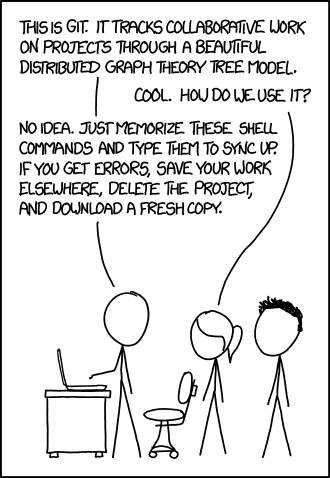
\includegraphics[height=.8\textheight]{img/xkcd-git.png}
\end{center}
\end{frame}
\begin{frame}[label={sec:org48d3cb1}]{Fluxul de lucru GitHub\footnote{\url{https://guides.github.com/introduction/flow/}}}
\begin{center}
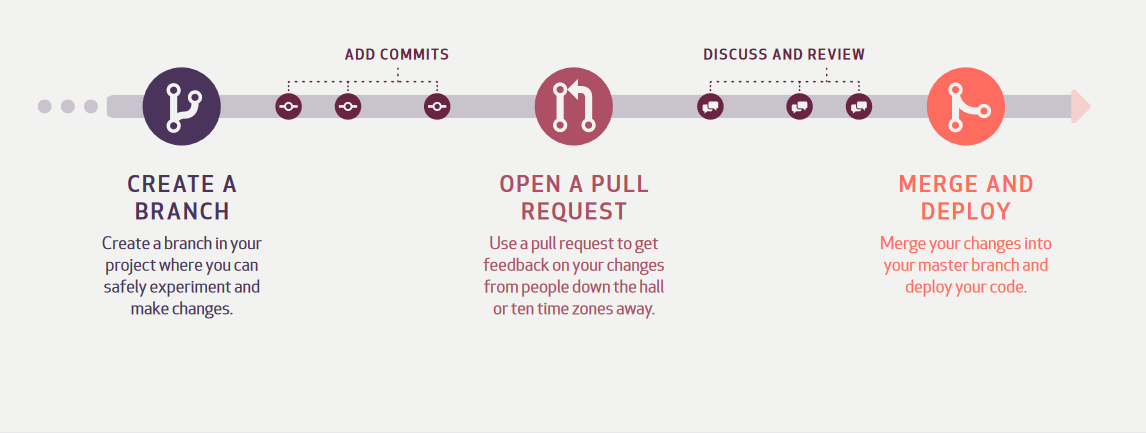
\includegraphics[width=\textwidth]{img/github-flow.png}
\end{center}
\end{frame}
\begin{frame}[label={sec:orgafaea58},fragile]{Fluxul de lucru GitHub}
 Pentru proiectele la care aveți drepturi să faceți modificări:
\begin{itemize}
\item Creați o ramură nouă,
\item Implementați cerințele prin \alert{modificări multiple și atomice},
\item Creați un \alert{Pull Request} din ramura nouă,
\item Revizuiți și modificați dacă este cazul,
\item Îmbinați ramura nouă cu \texttt{master},
\item Livrați funcționalitatea adăugată.
\end{itemize}
\end{frame}
\begin{frame}[label={sec:org06f68ce},fragile]{Fluxul de lucru extins\footnote{\url{https://guides.github.com/activities/forking/}}}
 Pentru proiectele la care nu aveți dreptul să faceți modificări:
\begin{itemize}
\item Creați un \texttt{fork} al proiectului,
\item Adăugați modificările necesare în \texttt{fork}-ul propriu (folosing fluxul de lucru de mai sus),
\item Creați un \texttt{Pull Request} din \texttt{fork}-ul propriu,
\item Adăugați modificări suplimentare dacă este cazul
\item O persoană desemnată va decide dacă modificările vor fi acceptate sau nu.
\end{itemize}
\end{frame}
\begin{frame}[label={sec:org06d006c}]{Descrierea modificărilor\footnote{\url{https://xkcd.com/1296/}}}
\begin{center}
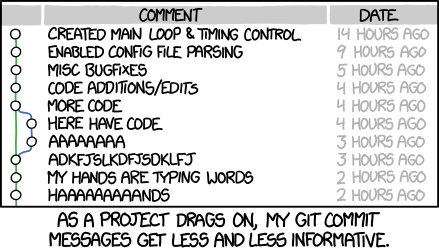
\includegraphics[width=.7\textwidth]{img/xkcd-git-commit.png}
\end{center}
\end{frame}
\begin{frame}[label={sec:org3d7e834}]{Ghid pentru descrierea modificărilor\footnote{\url{https://chris.beams.io/posts/git-commit/}}}
\begin{itemize}
\item Lăsați o linie goală între sumar și restul descrierii.
\item Sumarul trebuie să aibă maxim 50 caractere.
\item Scrieți conform regulilor de gramatică și ortografie:
\begin{itemize}
\item Începeți propozițiile cu majusculă,
\item Nu puneți punct după sumar.
\end{itemize}
\item Descrierea trebuie să explice \alert{ce} și \alert{de ce} a fost modificat; nu \emph{cum}.
\end{itemize}
\end{frame}
\section{Ecosistemul \texttt{NuGet}}
\label{sec:orgb351a84}
\begin{frame}[label={sec:orgcd05010},fragile]{Ce este \texttt{NuGet}?}
 \begin{itemize}
\item Aplicație utilitară pentru integrarea bibliotecilor oferite de terți în soluție/proiect.
\item Facilitează instalarea pachetelor și a pachetelor de care acestea depind.
\item Facilitează ștergerea și actualizarea pachetelor.
\end{itemize}
\end{frame}
\begin{frame}[label={sec:org965a327},fragile]{Ce este un \texttt{pachet NuGet}?}
 \begin{itemize}
\item O arhivă cu extensia schimbată din \texttt{.zip} în \texttt{.nupkg}.
\item Conține bibliotecile necesare (fișierele \texttt{.dll}) și metadate.
\end{itemize}
\end{frame}
\begin{frame}[label={sec:org0302c7f},fragile]{Pachetele \texttt{NuGet}}
 \begin{itemize}
\item Cele publice se găsesc pe \url{https://www.nuget.org/}.
\item Pentru pachetele private sunt necesare servere dedicate.
\end{itemize}
\end{frame}
\section{Principiile \texttt{SOLID}}
\label{sec:orgb90eed9}
\begin{frame}[label={sec:org7cd0d8a}]{SOLID}
\begin{description}
\item[{S}] Single Responsibility Principle
\item[{O}] Open-Closed Principle
\item[{L}] Liskov Substitution Principle
\item[{I}] Interface Segregation Principle
\item[{D}] Dependency Inversion Principle
\end{description}
\end{frame}
\begin{frame}[label={sec:org582b83c},fragile]{Context}
 Vrem să simulăm tranzacții financiare modelând diverse tipuri de conturi bancare (\texttt{Debit}, \texttt{Credit} etc.) precum și operațiunile care se fac asupra acestora.

Mai multe detalii în cursul II.
\end{frame}
\begin{frame}[label={sec:org21097bd}]{Single Responsibility Principle}
\begin{block}{Single Responsibility Principle}
Fiecare modul trebuie să fie responsabil pentru un singur aspect legat de funcționalitatea oferită de sistemul software. Mai mult, acel aspect trebuie să fie încapsulat în întregime de modulul responsabil\footnote{\url{https://en.wikipedia.org/wiki/Single\_responsibility\_principle}}.
\end{block}
\end{frame}
\begin{frame}[label={sec:orga1204be}]{Open-Closed Principle}
\begin{block}{Open-Closed Principle}
Părțile componente ale unui sistem software trebuie să fie ușor de extins dar greu de modificat\footnote{\url{https://en.wikipedia.org/wiki/Open/closed\_principle}}.
\end{block}
\end{frame}
\begin{frame}[label={sec:orgdc66d77}]{Liskov Substitution Principle}
\begin{block}{Liskov Substitution Principle}
Obiectele unui sistem software trebuie să fie substituibile de către instanțe ale unor subtipuri de obiecte, fără ca substituția să afecteze corectitudinea sistemului\footnote{\url{https://en.wikipedia.org/wiki/Liskov\_substitution\_principle}}.
\end{block}
\end{frame}
\begin{frame}[label={sec:orge089924}]{Interface Segregation Principle}
\begin{block}{Interface Segregation Principle}
Interfețele trebuie să fie mici și specifice contextului de utilizare; nu mari și generale\footnote{\url{https://en.wikipedia.org/wiki/Interface\_segregation\_principle}}.
\end{block}
\end{frame}
\begin{frame}[label={sec:orgabaa785}]{Dependency Inversion Principle}
\begin{block}{Dependency Inversion Principle}
Modulele unui sistem software trebuie să depindă de reprezentări abstracte și nu de implementări concrete\footnote{\url{https://en.wikipedia.org/wiki/Dependency\_inversion\_principle}}.
\end{block}
\end{frame}
\section{Încheiere}
\label{sec:orga54c08b}
\begin{frame}[label={sec:orgf85c2e1},fragile]{Recapitulare --- fluxul de lucru Git}
 \begin{itemize}
\item O ramură nouă pentru o cerință (\texttt{branch per feature})
\item Modificări atomice
\item Sincronizări frecvente
\item \texttt{Pull-Request} și îmbinare în \texttt{master}
\end{itemize}
\end{frame}
\begin{frame}[label={sec:org6833631},fragile]{Recapitulare --- \texttt{NuGet}}
 Este indicat să folosim \texttt{NuGet} pentru adăugarea de biblioteci în soluție/proiect.
\end{frame}
\begin{frame}[label={sec:org3c35317},fragile]{Recapitulare --- \texttt{SOLID}}
 \begin{itemize}
\item \alert{Single Responsibility Principle}
\item \alert{Open-Closed Principle}
\item \alert{Liskov Substitution Principle}
\item \alert{Interface Segregation Principle}
\item \alert{Dependency Inversion Principle}
\end{itemize}
\end{frame}
\end{document}